\section{Años 90's: Despegue de las ómicas}

Aunque las secuencias de proteínas fueron un punto de partida dada su temprana disponibilidad, la secuenciación de ADN también fue avanzando aceleradamente y ya en la década de los 90's tenía gran desarrollo.
Ejemplo de esto fue la secuenciación del primer genoma completo de un organismo independiente (no parásito) en 1995, \textit{Haemophilus influenzae} \cite{fleischmannWholegenomeRandomSequencing1995}.
Pero aún más importante fue el lanzamiento de unos de los proyectos más ambiciosos en la historia de la Biología: el Proyecto del Genoma Humano.

\begin{figure}[tb]
  \centering
  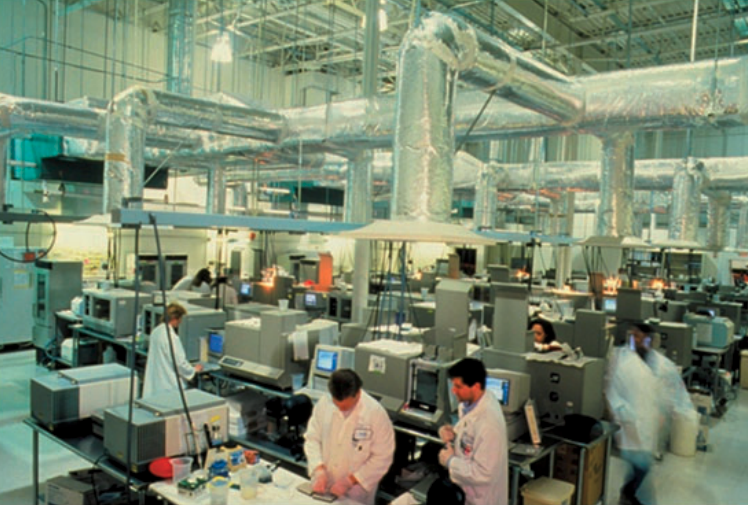
\includegraphics[width=0.7\columnwidth]{images/human_genome_project.png}
  \caption{Secuenciación a escala industrial durante Proyecto del Genoma Humano. Fuente \cite{gauthierBriefHistoryBioinformatics2019}}
  \label{fig:human_genome_project}
\end{figure}

El proyecto, financiado principalmente por el gobierno de los Estados Unidos, comenzó en 1991 (figura \ref{fig:human_genome_project}).
Una década, 2.7 miles de millones de dólares y 3 mil millones de pares de bases después \cite{web:HGP_FAQ}, se presentaba la primera versión de un genoma humano de referencia \cite{internationalhumangenomesequencingconsortiumFinishingEuchromaticSequence2004}.
Este acontecimiento es considerado el punto de partida de lo que se conoce como la era de las \textit{ómicas} en la Biología.

Las ómicas son un conjunto de disciplinas que se especializan en el estudio de los componentes y relaciones que conforman un organismo vivo (figura \ref{fig:Central_Dogma}).
Estas disciplinas se caracterizan por su carácter total, no se estudia un componente en particular, se intenta alcanzar a todos en el organismo en cuestión.
Entre ellas están las que estudian las diferentes especies moleculares, la genómica (el ADN), la transcriptómica (el ARN), la proteómica (las proteínas), la metabolómica (los intermediarios metabólicos), etc.
Además están las que estudian otros aspectos como la epigenética (estudio de los patrones de metilación del ADN), la fenómica (estudio de todos los fenotipos mutantes), la regulómica (los componentes moleculares regulatorios) y muchas más \cite{evansDesignerScienceOmic2000}.
El patrón es simple, ``algo biológicamente interesante'' + ``ómica''.
Estas, casi siempre surgen cuando se desarrolla alguna técnica experimental que permite obtener los datos requeridos a gran escala.

\begin{figure}[tb]
  \centering
  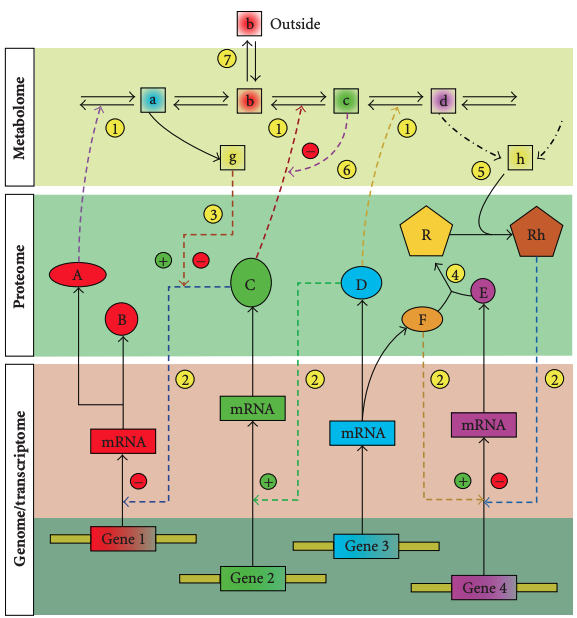
\includegraphics[width=0.7\columnwidth]{images/Central_Dogma.png}
  \caption{
      (\textit{Figura en inglés})
      El Dogma Central de la Biología Molecular y las ómicas.
      Con el desarrollo de las ómicas se pretende construir un mapa detallado que comprenda todos los componentes celulares y sus interrelaciones, cientos de miles de componentes y millones de interacciones.
      Fuente \cite{likicSystemsBiologyNext2010a}}
  \label{fig:Central_Dogma}
\end{figure}

En estas disciplinas los conceptos computacionales no son solo fundamentales, sino nativos.
Junto con los elaborados procedimientos experimentales, nuevas tecnologías y algoritmos deben ser creados para hacer frente a la cantidad de datos sin precedentes que se generan.
Un papel muy importante en las etapa inicial de desarrollo de las ómicas lo jugó la evolución de la red mundial de computadoras \cite{gauthierBriefHistoryBioinformatics2019}.
A principios de los 90's Tim Berners-Lee crea la \textit{World Wide Web}, un sistema internacional de documentos interconectados, lo que se considera como el comienzo de la internet \cite{web:WWW}.
Esta red ha jugado, y juega, un papel esencial a la hora de facilitar la colaboración a gran escala necesaria en proyectos de gran magnitud.
Desde el almacenamiento hasta la publicación y acceso de los resultados, la Biología es ``subida a la nube''.

